\documentclass[10pt,twocolumn]{article}


\usepackage[utf8]{inputenc}

\usepackage{lecture-notes-template/zsfgv}
\usepackage{lipsum}
\usepackage{multicol}

\graphicspath{{img/}}

\raggedbottom

\begin{document}

\part{Natural Language Processing}

\section{Introduction}

\paragraph{\textit{Challenges}}
\begin{itemize}
\item Complicated structure in sentence
\item Syntactic ambuigities (``\textit{time flies like an arrow}'',
  ``\textit{get the cat with the gloves}'').
\item Metaphores, humor, irony, ...
\item Semantics can be very rich and dependent on context, not easy to
  distuingish
\item Language requries knowledge about the world
\item Hard to really formalise the notion of ``meaning''
\end{itemize}

\paragraph{\textit{Basic approach}} Gather information on word based on its
context. Given a large text corpus, we can assume this to be meaningful
statistics.

\paragraph{\ild{Zipf's Law}} The number of elements with a given frequency
follows a power law distribution. That is, there is a small number of elements
which appear very often and the majority of elements appears rarely. In its most
simple form, the probability of the $n$-th most common word $p(n)$ is
\begin{align*}
  p(n) = \nicefrac{1}{n}
\end{align*}
\begin{figure}[h]
  \centering
  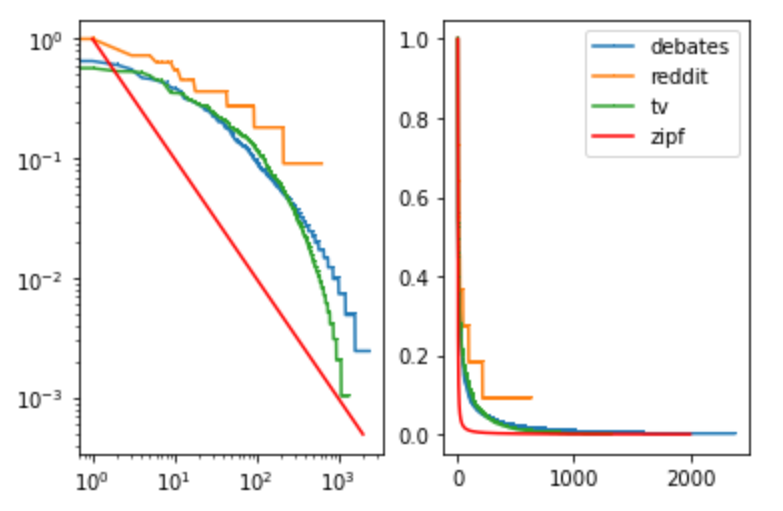
\includegraphics[width=0.8\linewidth]{zipf.png}
\end{figure}

\paragraph{\ild{Elements of language}} We can have different points of view on
language:
\begin{itemize}
\item Phonetics (sound)
\item Grammar
\begin{itemize}
\item Phonology
\item Morphology
\item Syntax
\end{itemize}
\item Semantics (meaning)
\end{itemize}

\paragraph{\ild{Morphology}} How words are built up from smaller meaningful
units, for instance \textit{un-lady-like}, \textit{dog-s}
\begin{itemize}
\item \textbf{\ild{Inflection}} -- variation in the form of a word (usually affix)
  that expresses a grammatical contrast
  \begin{itemize}
  \item adds tense, number, person, mood, aspect, etc
  \item e.g. \textit{run}$\rightarrow$ \textit{run} | \textit{running} 
  \item does not change word class
  \end{itemize}
\item \textbf{\ild{Derivation}} -- formation of a new word from another
  \begin{itemize}
  \item e.g. nominalization (\textit{computer}$\rightarrow$\textit{computerization})
  \item e.g. formation of adjectives (\textit{computational}, \textit{clueless})
  \item changes word class
  \end{itemize}
\end{itemize}

\paragraph{\textit{Morphemes}}
\begin{itemize}
\item \textbf{\ild{Root}} -- equivalence class of a word when all affixes are
  removed; not further decomposable into meaningful elements.
\item \textbf{\ild{Stem}} -- part of word that never changes when
  morphologically inflected, \iln{ i.e. without affixes describing tense, number,
  person, ... }
\item \textbf{\ild{Lemma}} -- Base form of word
\item From \textit{produced}, lemma is \textit{produce} but stem is \textit{produc}
\end{itemize}


\section{Tokenization}
 
\paragraph{\ild{Token}} an individual occurence of a word (as opposed to a
vocabulary/dictionary item)

\paragraph{\textit{Challenges}}
\begin{itemize}
\item Keep abbreviations, dates, numbers as single tokens
\item distuingish abbreviations from words
\item names and phrases (\textit{queen of england}, \textit{TU Wien})
\item compound words
\item apostrophes, umlauts, etc and other linguistic characteristics
\item encoding issues like RTL/LTR
\end{itemize}

\paragraph{\ila{Maximum Matching algorithm}} Use a dictionary of known terms.
Take the longest prefix of the input string that matches a dictionary item. Does
not always make sense (\textit{``Theta bled own there''}).

\section{Stemming}

\paragraph{\textit{Stemming/Lemmatization}} reduce tokens to equivalence
classes. Usually to gather words that are morphologically different but
semantically quite similar to the same set, i.e. to improve comparability. 

\paragraph{\ila{Porter Stemmer} } Rules for stripping suffixes. Applicability of
rules is based on \textit{measure} of a word $w$, which is the number $m$ s.t.
$w=C(VC)\{m\}V$ where $C,V$ are arbitrary sequences of consontants, vowels,
resp. --- Indeed reduces the words to their \textit{stems}.

\paragraph{\ila{WordNet \textsc{Morphy}} }
\begin{itemize}
\item Has  •  a sophisticated set of rules about inflections  • exception list
\item Checks the result of transformation against an extensive dictionary
\end{itemize}

\paragraph{\iln{Note}} \textsc{Morphy} reduces to \textit{lemmas}, while
\textsc{Porter} reduces to \textit{stems}.

\begin{itemize}
\item \textbf{\ild{Over-stemming}} Two words are reduced to the same root when
  they should not be
\item \textbf{\ild{Under-stemming}} Should be reduced to the same root but are not.
\end{itemize}


\section{POS-Tagging}

Given some input text and some tags (usually word types such as \textit{noun},
\textit{verb}, etc.), want to assign tags to tokens. (\textit{Sequence
  classification problem}).

Tagging can help with other procedures such as stemming, NER, parsing, ...

\paragraph{\ild{Def.}} Can divide words into two different classes
\begin{itemize}
  \item \textbf{\ild{Closed class}} --- can enumerate all members, e.g.
    determiners, pronouns, prepositions, ...
\item \textbf{\ild{Open class}} --- don't know all members, e.g. nouns, verbs,
  adjectives, ...
\end{itemize}

\paragraph{\iln{Note}}
\begin{itemize}
\item A single term (dictionary entry) can have different optimal POS-tags
  depending on its context.
\item Tagging helps to resolve ambiguities that exist on term-level (.e.g
  \textit{leaves} as \textsc{NN} or as \textsc{VB})
\item Tagging removes unnecessary distinctions e.g. all personal pronouns are
  \textsc{PRP}, determiners
\item Naive method (assigning most frequent tag in training data to term)
  already has 90\% accuracy.
\end{itemize}

\paragraph{\ild{Def.}}
\begin{itemize}
\item \textbf{\ild{Informativeness}} --- Assignment of tag adds information,
  reduces ambuigity
\item \textbf{\ild{Specifiability}} --- Ease of mapping a term to a tag
\item \iln{Example}: Collapsing multiple related tags into one decreases
  informativeness, decreases specifiability.
\end{itemize}

\paragraph{\textit{Feature selection}} Can look at word-local features (term,
pre-, suffixes, capitalization); but very often the tag of a word depends on its
context in the sentence.

\paragraph{\textbf{Main techniques}}
\begin{itemize}
\item \ild{Probabilistic tagging} --- consider lexical frequencies of tag in
  training data -- good when large training corpora are available
\item \ild{Rule-based tagging} --- use rules based on linguistic understanding
  -- good to tailor solution to very specific problems
\end{itemize}

\subsection{Probabilistic tagging}

Consider the definition of \ild{ conditional probability }
\begin{align*}
  P(A|B) = \frac{P(A,B)}{P(B)} 
\end{align*}
This gives rise to the \ild{chain rule}
\begin{align*}
  \Rightarrow P(A,B) = P(A|B) \cdot P(B)
\end{align*}
or, more generally
\begin{align*}
  P(w_1, ..., w_n) = \prod P(w_i~|~w_1, ..., w_{i-1})
\end{align*}
The problem here is that we cannot realistically obtain all the components of
the product because there are way too many possible sequences of words. Instead,
we employ the \ild{Markov assumption} that says that we can estimate the
probabilities by only consiering only the $k$ preceding terms
\begin{align*}
  P(w_i ~|~ w_1 ..., w_{i-1}) \approx P(w_i ~|~ w_{i-k}, ..., w_{i-1})
\end{align*}

For $k=1$, this yields the \ild{unigram model}, for $k=2$ the \ild{bigram model}
(i.e. $P(w_i | w_{i-1})$).

$n$-gram modelling is insufficient because language has \textit{long-distance depenencies}.

\paragraph{\ila{Unigram Tagger} } Assume that a unigram model generates the
current tagging. 

Assign a token $w$ its most frequent tag, i.e.
\begin{align*}
  t(w) := \argmax_t P(t~|~w)
\end{align*}
\textit{Improvement}: Use Bayes' formula, i.e. $P(A|B) = \frac{P(B|A)P(B)}{P(B)}$,
omitting the quotient:
\begin{align*}
  t(w) := P(t~|~w) = \argmax_t P(t) \cdot P(w~|~t)
\end{align*}

\paragraph{\textit{ \todo }} example

\paragraph{\ila{$n$-gram tagger} } Use information about the previous $n$
tokens in addition to information about current token. Can have \ild{word-based}
and \ild{tag-based} (tags are more common, training data covers more ground).

Assume a bigram language model (generating the sequence of POS-tags).

Pick the tag $t_i$ for word $w_i$ that maximises
\begin{align*}
  P(t_i ~|~ t_{i-1}) \cdot P(w_i~|~t_{i-1})
\end{align*}

For finding $P(t_i~|~t_{i-1})$, use the \ild{Maximum Likelihood Estimate} (where
$c$ is the count of observations)
\begin{align*}
  P(t_i | t_{i-1}) \approx \frac{c(w_{i-1}, w_i)}{c(w_{i-1})}
\end{align*}
\iln{(Use start and end symbols to be able to calculate probs for first and last
  words)}

% For $n=2$, can imagine a twodimensional lookup table:
% \begin{align*}
%   \text{previously seen POS-tag} \times \text{current word} \rightarrow 
% \end{align*}

\paragraph{\textit{\todo}} example


\subsection{Rule-based tagging}

Try to incorporate linguistic insight.

\paragraph{\ila{Brill tagger} }
\begin{enumerate}
\item Tag each word using a \ild{ baseline tagger } (e.g. unigram tagger, i.e.
  most common tag)
\item Apply patches that improve the result
  \begin{itemize}
  \item e.g. \textit{if one of the two preceding words is a determiner, change
      the tag from verb to noun}
  \item Based on training data, compute the error between any two
    should-be/is-assigned: $(t_a, t_b, \mathit{freq})$.
  \item For each error triple, apply the patch that results in the greatest
    improvement, apply it.
  \item Repeat until no further improvement is possible.
  \end{itemize}

\end{enumerate}



\section{Parsing}

\pagebreak
\part{Similarity Measures}

\pagebreak
\part{Language Modelling}

\pagebreak
\part{Text Data Mining}

\pagebreak
\part{Opinion Mining \& Information Extraction}

\section{Information Extraction}

to extract  • the entities and  • relationships between such entities (i.e.
clear, factual information)

\subsection{Named Entity Extraction}

used for  • summarizing text  • answering questions  • integrating into knowlege
bases  • associating information (e.g. sentiments) to sentiments (e.g. of parts
of printer in question)

Possible types of entities  • location  • time  • person  • ...

\paragraph{\textit{Supervised learning models}} Based on labelled training
sequences (of tokens), train a classifier to predict labels (\textit{Sequence
  Labelling Problem})
\begin{itemize}
\item new data must fit training data
\item time-consuming
\end{itemize}

To make this easier, use features that go beyond single tokens, e.g. context
window of $k$ words.

\paragraph{\textit{Sequence Labelling}}  • reminiscent to POS-tagging  • assuming
that label is dependent on context. Typical models are  • Markov models  •
Conditional Random Fields  • Bidirectional LSTMs

Once we have identified the entities, we'd like to find relationships between
them (e.g. triples of operators \textit{is-a}, \textit{daughter-of}, ...)
\iln{(Can save these triples in a knowledge base e.g. for question-answering; cf
  \textsc{Rdf}-triples)}.

\paragraph{\textit{Relationship Extraction}} Try to find type of relationship
between two entitties. Possibilities
\begin{itemize}
\item Extract \textsc{Rdf} triples from large corpora like Wikipedia
\item Use (specialised) ontologies / knowledge bases (for ex. medical applications)
\end{itemize}
Methods to extract information:
\begin{itemize}
\item handwritten rules -- e.g. \textit{``Y such as X'', ``X, especially Y'',
    ``X, including Y'' all express an \textit{is-a}-relationship}. -- there can
  be more specific relations that only make sense between certain types of
  entities (e.g. \textit{cures(drug, disease)}) -- pros:  • precise  • can be
  tailored to specific domains -- cons:  • low recall  • high effort
\item supervised,
\item unsupervised machine learning.
\end{itemize}

semi-supervised learning: extract less common patterns based on training corpus?






\pagebreak
\part{Question Answering \& Text Summarization}


\end{document}